\chapter{Water in All Its States}\label{ch:g6:water-states}

You have chased water through its states since your second school
year: ice, water, steam; \omterm{def:g6:water-states:changes}{melting} snowmen and misty windows. This
year the chase becomes bookkeeping. When ice \omterm{def:g2:ice-water-steam:meltfreeze}{melts}, is any stuff
lost? When water \omterm{def:g2:ice-water-steam:meltfreeze}{freezes}, why do pipes burst? With balances and
cylinders in hand, we audit all three of water's states.

\section{The three states, with proper labels}

\begin{definition}[The six changes of state]\label{def:g6:water-states:changes}
Between its three states, water has six doors, each with its
scientific name:
\begin{enumerate}
  \item \omterm{def:g3:solids-liquids-gases:solid}{solid} $\to$ \omterm{def:g3:solids-liquids-gases:liquid}{liquid}: \emph{melting}\index{melting};
        \omterm{def:g3:solids-liquids-gases:liquid}{liquid} $\to$ \omterm{def:g3:solids-liquids-gases:solid}{solid}:
        \emph{solidification}\index{solidification} (freezing);
  \item \omterm{def:g3:solids-liquids-gases:liquid}{liquid} $\to$ \omterm{def:g3:solids-liquids-gases:gas}{gas}: \emph{vaporization}\index{vaporization}
        --- roaring fast at the boil, quiet and cool as
        evaporation; \omterm{def:g3:solids-liquids-gases:gas}{gas} $\to$ \omterm{def:g3:solids-liquids-gases:liquid}{liquid}:
        \emph{condensation}\index{condensation};
  \item \omterm{def:g3:solids-liquids-gases:solid}{solid} $\to$ \omterm{def:g3:solids-liquids-gases:gas}{gas} directly:
        \emph{sublimation}\index{sublimation}, and \omterm{def:g3:solids-liquids-gases:gas}{gas} $\to$ \omterm{def:g3:solids-liquids-gases:solid}{solid}
        directly --- rarer doors, but real: frost feathers on a
        freezing window grow straight from invisible vapor,
        skipping the \omterm{def:g3:solids-liquids-gases:liquid}{liquid} entirely.
\end{enumerate}
\end{definition}

\begin{omfigure}
\begin{tikzpicture}[scale=0.85]
  \node[draw, thick, omDef, font=\small, minimum width=1.9cm,
    minimum height=0.85cm] (ice) at (1.2,0) {ice};
  \node[draw, thick, omDef, font=\small, minimum width=1.9cm,
    minimum height=0.85cm] (wat) at (5.7,0) {water};
  \node[draw, thick, omDef, font=\small, minimum width=1.9cm,
    minimum height=0.85cm] (vap) at (10.2,0) {vapor};
  \draw[-Stealth, very thick, omThm] (2.25,0.28) -- (4.65,0.28);
  \node[above, font=\footnotesize, omThm] at (3.45,0.42) {melting};
  \draw[-Stealth, very thick, omDef] (4.65,-0.28) -- (2.25,-0.28);
  \node[below, font=\footnotesize, omDef] at (3.45,-0.42)
    {solidification};
  \draw[-Stealth, very thick, omThm] (6.75,0.28) -- (9.15,0.28);
  \node[above, font=\footnotesize, omThm] at (7.95,0.42)
    {vaporization};
  \draw[-Stealth, very thick, omDef] (9.15,-0.28) -- (6.75,-0.28);
  \node[below, font=\footnotesize, omDef] at (7.95,-0.42)
    {condensation};
  \draw[-Stealth, very thick, omThm]
    (1.2,0.6) .. controls (3.0,2.1) and (8.4,2.1) .. (10.1,0.6);
  \node[above, font=\footnotesize, omThm] at (5.7,1.85)
    {sublimation};
\end{tikzpicture}

{\small Water's six doors, with their proper names. Warmth drives
the red doors; cold drives the blue.}
\end{omfigure}

\begin{example}[Doors all around you]\label{ex:g6:water-states:doors}
Morning frost \omterm{def:g6:water-states:changes}{melting} off the grass; laundry evaporating on the
line; a cold \omterm{def:g5:mirrors-reflection:reflection}{mirror} condensing your shower's vapor; the freezer
solidifying tomorrow's ice cubes; frost feathers grown overnight on
the pane. One substance, six doors, all within a day of ordinary
life --- name them and you own them.
\end{example}

\section{The audit: is stuff lost?}

\begin{method}[Weighing a change of state]\label{met:g6:water-states:weigh}
Put the question to the balance:
\begin{enumerate}
  \item pour some water into a small plastic bottle, screw the cap
        tight, dry the outside;
  \item weigh it: say \qty{368}{g} --- write it down;
  \item lay it in the freezer overnight: \omterm{def:g6:water-states:changes}{solidification};
  \item weigh the frozen bottle at once (dry off any frost).
\end{enumerate}
The balance answers: \qty{368}{g}, to the \omterm{def:g3:measuring-mass:units}{gram}. \omterm{def:g2:ice-water-steam:meltfreeze}{Melt} it back on
the windowsill and weigh again: \qty{368}{g}. The state changed
twice; the stuff never blinked.
\end{method}

\begin{proposition}[Mass survives changes of state]\label{prop:g6:water-states:mass}
A change of state changes a substance's appearance, not its
amount: the \omterm{def:g3:measuring-mass:mass}{mass} before equals the \omterm{def:g3:measuring-mass:mass}{mass} after, exactly. \omterm{def:g6:water-states:changes}{Melting},
freezing, boiling in a sealed pot, condensing --- through every
door, the balance reads the same. (Leave the cap off, though, and
vapor drifts away with its \omterm{def:g3:measuring-mass:units}{grams}: the stuff still exists, but your
audit no longer contains it.)
\end{proposition}

\begin{example}[Where the puddle's grams went]\label{ex:g6:water-states:puddle}
A \qty{300}{g} puddle dries up. Vanished? Weighed nothing? No:
\qty{300}{g} of water now ride the \omterm{def:g2:air-around-us:air}{air} as invisible vapor, every
\omterm{def:g3:measuring-mass:units}{gram} intact --- some to fall as next week's rain. Evaporation
fools the eye, never the bookkeeping. The chalk line of your
childhood puddle experiment was an audit; now it has numbers.
\end{example}

\section{The audit: is room kept?}

\begin{proposition}[Water swells as it freezes]\label{prop:g6:water-states:volume}
\omterm{def:g3:measuring-mass:mass}{Mass} survives the doors --- \omterm{def:g6:mass-and-volume:volume}{volume} does not. Water is a curious
substance: turning \omterm{def:g3:solids-liquids-gases:solid}{solid}, it \emph{expands}. A \omterm{def:g6:mass-and-volume:volume}{litre} of water
makes about $1.1$ \omterm{def:g6:mass-and-volume:volume}{litres} of ice: same \omterm{def:g3:measuring-mass:mass}{mass}, about a tenth more
room. Most substances shrink when they solidify; water swells ---
and that oddity redraws landscapes.
\end{proposition}

\begin{omfigure}
\begin{tikzpicture}[scale=0.85]
  \draw[thick] (1.2,0) -- (1.2,3.4) (3.0,0) -- (3.0,3.4)
    (1.2,0) -- (3.0,0);
  \fill[omDef, opacity=0.25] (1.2,0.05) rectangle (3.0,2.2);
  \draw[omDef, very thick] (1.2,2.2) -- (3.0,2.2);
  \node[below, font=\small] at (2.1,-0.3)
    {before: water, \qty{368}{g}};
  \draw[thick] (7.0,0) -- (7.0,3.4) (8.8,0) -- (8.8,3.4)
    (7.0,0) -- (8.8,0);
  \fill[omDef, opacity=0.45] (7.0,0.05) rectangle (8.8,2.42);
  \draw[omDef, very thick] (7.0,2.42) -- (8.8,2.42);
  \draw[dashed, omExo] (7.0,2.2) -- (8.8,2.2);
  \node[below, font=\small] at (7.9,-0.3)
    {after freezing: ice, still \qty{368}{g}};
  \draw[-Stealth, omThm, thick] (5.0,2.6) -- (6.8,2.45);
  \node[above, font=\small, omThm] at (5.0,2.65)
    {the level rose: more room, same mass};
\end{tikzpicture}

{\small The frozen bottle: the balance unchanged, the level higher.
Freezing keeps the stuff and demands more room.}
\end{omfigure}

\begin{example}[The burst pipe and the cracked mountain]\label{ex:g6:water-states:burst}
Forgotten in the freezer, a full glass bottle of water cracks: the
swelling ice needs its extra tenth of room and takes it, glass or
no glass. Winter does the same to plumbing --- water freezing in a
pipe bursts it as surely as a hammer --- and to mountains: rain
seeps into rock cracks, \omterm{def:g2:ice-water-steam:meltfreeze}{freezes} at night, swells, and wedges the
crack wider. Year by year, \omterm{def:g2:ice-water-steam:meltfreeze}{freeze} by \omterm{def:g2:ice-water-steam:meltfreeze}{freeze}, the odd little
swelling of \cref{prop:g6:water-states:volume} splits boulders and
crumbles peaks.
\end{example}

\begin{remark}[Why ice floats]\label{rem:g6:water-states:floats}
The same oddity answers a question you asked years ago at bath
time. Ice holds a \omterm{def:g6:mass-and-volume:volume}{litre}'s stuff in $1.1$ \omterm{def:g6:mass-and-volume:volume}{litres} of room: for equal
room, ice is \emph{lighter} than water --- so ice \omterm{def:g1:floating-and-sinking:words}{floats} on its
own \omterm{def:g3:solids-liquids-gases:liquid}{liquid}. Icebergs ride the sea, ponds \omterm{def:g2:ice-water-steam:meltfreeze}{freeze} from the top down
(saving the fish beneath), and your lemonade's cubes bob instead
of sinking. Few substances \omterm{def:g1:floating-and-sinking:words}{float} on themselves; life on frozen
ponds is glad water does.
\end{remark}

\section{The water cycle, audited}

\begin{example}[The great round trip, with vocabulary]\label{ex:g6:water-states:cycle}
The childhood story of sea, cloud and rain now reads like a
ledger. The Sun's warmth drives \emph{\omterm{def:g6:water-states:changes}{vaporization}} from the seas
--- tonnes upon tonnes rise invisibly. High and cold, the vapor
\emph{\omterm{def:g2:ice-water-steam:evapcond}{condenses}} into cloud droplets; colder still, droplets
\omterm{def:g2:ice-water-steam:meltfreeze}{freeze} into snow. Snow piles into glaciers; glaciers \emph{\omterm{def:g2:ice-water-steam:meltfreeze}{melt}}
into rivers; rivers return every \omterm{def:g3:measuring-mass:units}{gram} to the sea. Around the whole
circuit, \cref{prop:g6:water-states:mass} holds: the \omterm{def:g4:solar-system:planet}{planet}
neither gains nor loses a drop --- the water in your glass has
sailed this loop since before the dinosaurs.
\end{example}

\begin{omfigure}
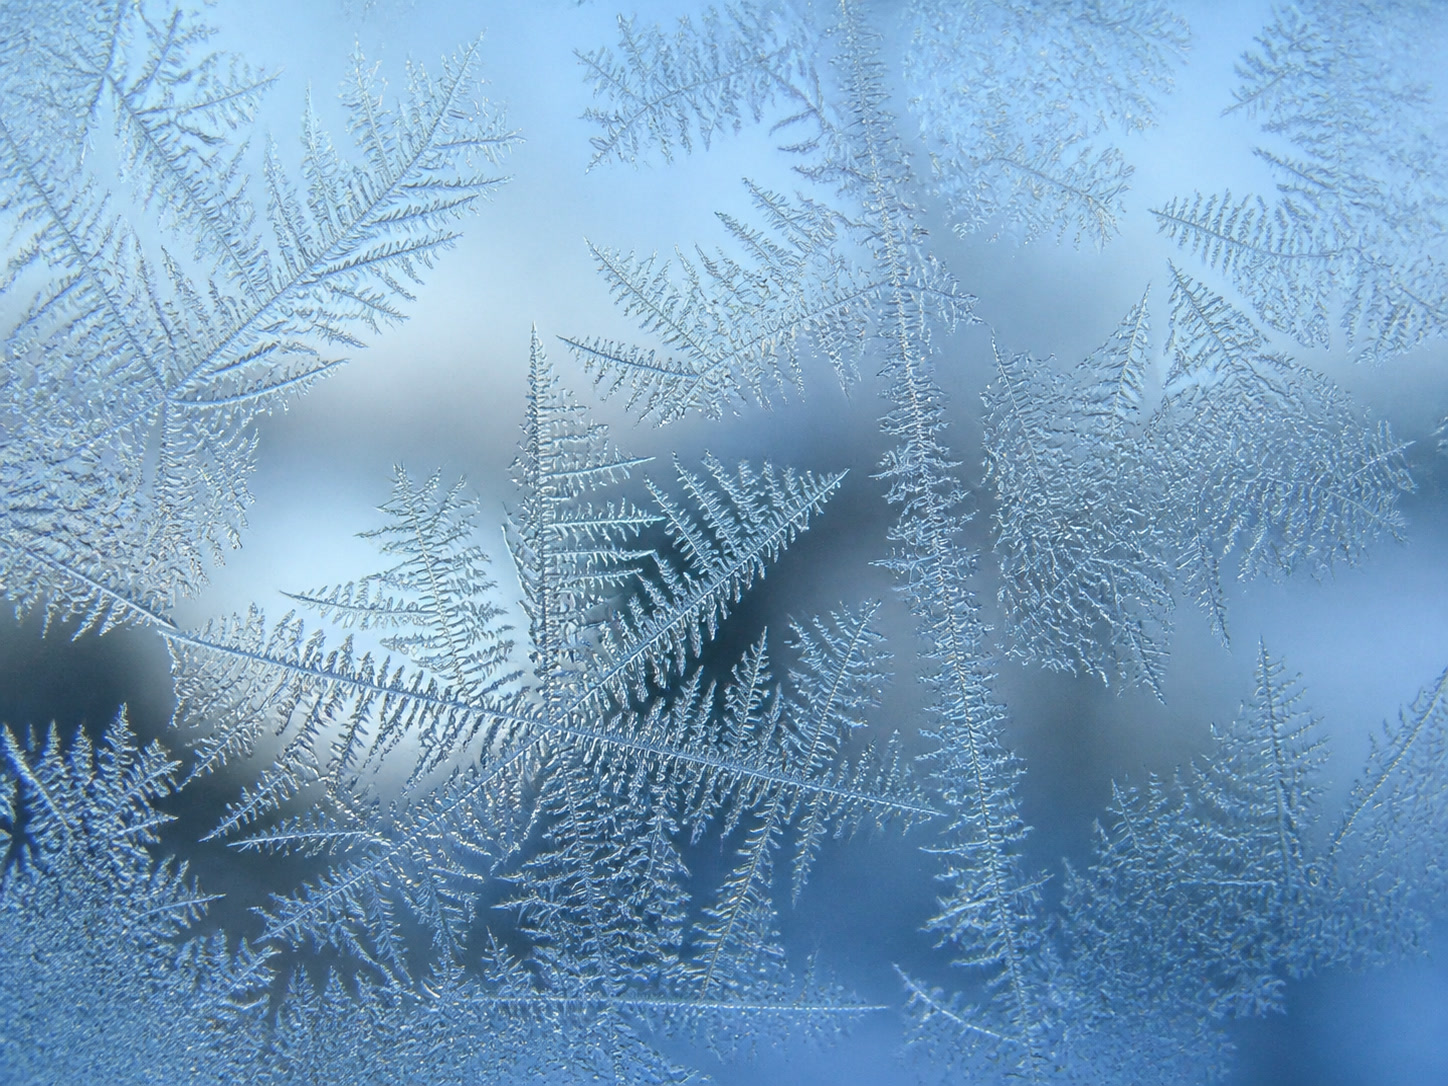
\includegraphics[width=0.5\linewidth]{images/book1/ai/g6-water-frost-window.jpg}

{\small Frost feathers on a freezing pane: water from the \omterm{def:g2:air-around-us:air}{air} built this ice overnight, straight onto the glass.}
\end{omfigure}

\section{Exercises}

\begin{exercise}[$\star$]\label{exo:g6:water-states:1}
Name the six doors of \cref{def:g6:water-states:changes}, each
with one everyday sighting.
\end{exercise}

\begin{exercise}[$\star$]\label{exo:g6:water-states:2}
Which door: dew forming on cold grass at dawn? \ a snowman
shrinking on a sunny \qty{-5}{\celsius} day, with no puddle
appearing? \ ice cubes clouding the freezer with ``smoke''?
\end{exercise}

\begin{exercise}[$\star$]\label{exo:g6:water-states:3}
A sealed bottle of water weighs \qty{412}{g}. It \omterm{def:g2:ice-water-steam:meltfreeze}{freezes} \omterm{def:g3:solids-liquids-gases:solid}{solid}
overnight. What does it weigh now, and which proposition answers?
\end{exercise}

\begin{exercise}[$\star$]\label{exo:g6:water-states:4}
In \cref{met:g6:water-states:weigh}, why must the bottle be capped
--- and why dried before each weighing?
\end{exercise}

\begin{exercise}[$\star$]\label{exo:g6:water-states:5}
A pot of water boils uncovered for ten minutes and its \omterm{def:g3:measuring-mass:mass}{mass} drops
by \qty{200}{g}. Was \omterm{def:g3:measuring-mass:mass}{mass} destroyed? Where are those \omterm{def:g3:measuring-mass:units}{grams}?
\end{exercise}

\begin{exercise}[$\star$]\label{exo:g6:water-states:6}
One \omterm{def:g6:mass-and-volume:volume}{litre} of water goes into the freezer. About what \omterm{def:g6:mass-and-volume:volume}{volume} of ice
comes out? Same question for the \omterm{def:g3:measuring-mass:mass}{mass}.
\end{exercise}

\begin{exercise}[$\star$]\label{exo:g6:water-states:7}
Why do water pipes burst in hard winters --- and why do gardeners
drain their outdoor taps in autumn?
\end{exercise}

\begin{exercise}[$\star$]\label{exo:g6:water-states:8}
Why does ice \omterm{def:g1:floating-and-sinking:words}{float} on water? Connect
\cref{prop:g6:water-states:volume} to the floating rule ---
lighter or heavier for the same room?
\end{exercise}

\begin{exercise}[$\star\star$]\label{exo:g6:water-states:9}
Tell the water cycle as a ledger: follow \qty{1}{kg} of sea water
around the full loop, naming each door it passes and stating its
\omterm{def:g3:measuring-mass:mass}{mass} at every stage.
\end{exercise}

\begin{exercise}[$\star\star$]\label{exo:g6:water-states:10}
A lemonade glass is filled to the very brim, ice cubes bobbing.
A guest worries it will overflow as the ice \omterm{def:g2:ice-water-steam:meltfreeze}{melts}. Use the two
audits (\omterm{def:g3:measuring-mass:mass}{mass} kept, ice's extra room given back) to reassure ---
or alarm --- the guest, with your reasoning.
\end{exercise}

\begin{exercise}[$\star\star$]\label{exo:g6:water-states:11}
Frost feathers appear on a freezing window pane overnight in a dry
room, with no rain and no wet pane at bedtime. Which door did the
water take, from where, and why is this door's name not
``freezing''?
\end{exercise}

\begin{exercise}[$\star\star\star$]\label{exo:g6:water-states:12}
Ponds \omterm{def:g2:ice-water-steam:meltfreeze}{freeze} from the top down. Explain the whole chain: why the
coldest water's ice forms \emph{at the surface} and stays there,
what the floating lid does to the \omterm{def:g5:heat-and-insulation:heat}{heat} flow beneath (an insulation
idea from last year), and why the fish below owe their winters to
water's strange swelling.
\end{exercise}

\section{Problem: A Kilogram Around the World}

\begin{problem}[{Weekend problem --- one kilogram of sea water on
its grand tour; six doors, three mountains, one unbroken
ledger}]\label{pb:g6:water-states:1}
We stamp an imaginary label on \qty{1}{kg} of sea water and follow
it for a year.

\medskip\noindent\textbf{Part I --- Up.}
\begin{enumerate}
  \item June: the Sun warms the sea surface and our \omterm{def:g3:measuring-mass:units}{kilogram} rises
        into the \omterm{def:g2:air-around-us:air}{air}, invisibly. Name the door it took.
  \item What is the \omterm{def:g3:measuring-mass:mass}{mass} of our (now invisible) \omterm{def:g3:measuring-mass:units}{kilogram} of
        water? Which
        proposition guarantees it?
  \item At \qty{3000}{m}, the \omterm{def:g2:air-around-us:air}{air} is cold: the water becomes a
        cloud of droplets. Name this door.
  \item Colder still, the droplets become snowflakes. Name that
        door --- \omterm{def:g6:water-states:changes}{solidification} --- and state the \omterm{def:g3:temperature-thermometers:temperature}{temperature} at
        which cloud droplets of pure water begin to \omterm{def:g2:ice-water-steam:meltfreeze}{freeze}.
\end{enumerate}

\medskip\noindent\textbf{Part II --- The glacier's ledger.}
Our \omterm{def:g3:measuring-mass:units}{kilogram} lands on a glacier and is pressed into glacier ice.
\begin{enumerate}[resume]
  \item As water, our \omterm{def:g3:measuring-mass:units}{kilogram} occupied \qty{1}{L}. About what
        \omterm{def:g6:mass-and-volume:volume}{volume} does it occupy as ice?
  \item The glacier's snout \omterm{def:g2:ice-water-steam:meltfreeze}{melts} in summer. Our \omterm{def:g3:measuring-mass:units}{kilogram} becomes
        meltwater: what is its \omterm{def:g3:measuring-mass:mass}{mass} now, and its \omterm{def:g6:mass-and-volume:volume}{volume} (back as
        \omterm{def:g3:solids-liquids-gases:liquid}{liquid} water)?
  \item On the way down the mountain, \qty{250}{g} of our
        \omterm{def:g3:measuring-mass:units}{kilogram} \omterm{def:g2:ice-water-steam:evapcond}{evaporates} from a sunlit waterfall pool. How much
        of the labeled water continues as \omterm{def:g3:solids-liquids-gases:liquid}{liquid} in the stream?
  \item Has the evaporated quarter left the audit? Say where its
        \qty{250}{g} are, and what door they will most likely take
        next.
\end{enumerate}

\medskip\noindent\textbf{Part III --- Home, and the books
balanced.}
\begin{enumerate}[resume]
  \item The stream's \qty{750}{g} reach the sea in October. The
        evaporated \qty{250}{g} fell as rain over the coast in
        August and ran to the sea in September. Add up what the
        sea got back of our \omterm{def:g3:measuring-mass:units}{kilogram}.
  \item Along the whole tour, our \omterm{def:g3:measuring-mass:units}{kilogram} was weightless exactly
        never --- but it was \emph{invisible} twice. At which
        stages, and in which state?
  \item A classmate objects: ``Snow is fluffy and \omterm{def:g1:light-and-shadows:source}{light} --- surely
        the \omterm{def:g3:measuring-mass:units}{kilogram} weighed less as snow.'' Untangle the mix-up
        with the right pair of words from this year.
  \item Write the tour as a chain of doors, in order, using only
        the six proper names of
        \cref{def:g6:water-states:changes}.
\end{enumerate}
\end{problem}
